\documentclass{article}
\usepackage[utf8]{inputenc}
\usepackage{kotex} % 한국어를 가능하도록 해주는 패키지 입니다. 
\usepackage[left=2.5cm,right=2.5cm,top=3cm,bottom=3cm,a4paper]{geometry} % 페이지 레이아웃 설정입니다. 
\usepackage{listings}  % 소스코드 작성에 필요한 패키지 입니다. 헤더파일이랑 비슷한 개념입니다. 
% 소스코드는 \begin{lstlisting} 이 사이에 써야됩니다. \end{lstlisting}
% 이건 주석입니다. 
% // 이건 개행입니다. 
% \indent 이건 들여쓰기입니다. 
% 논문 링크는 references.bib에서 수정한 후에 
% 이 파일로 돌아와서 해당 부분에 \citep[이름] 코드를 붙여야합니다. 
% 사진의 경우 import 후 30번째 줄을 참고하시면 됩니다. 

\title{Darknet YOLO API}
\author{이대경, 김한섭, 강일송 }
\date{2017학년도 2학기 오픈소스 Team Project}

\usepackage{natbib}
\usepackage{graphicx}

\begin{document}

\maketitle

\section{You Only Look Once}

\indent YOLO시스템은 최첨단 실시간 물체 감지 시스템이다.
기존의 탐지시스템은 Repurpose classifiers 혹은 Localizers를 사용하여 탐지를 수행하였습니다. 이 방법은 모델의 여러 위치에 격자 이미지를 적용하는 방식이며 격자 중 높은 일치도를 보인 물체를 탐지합니다. 하지만 YOLO는 하나의 신경망을 전체 이미지에 적용하는 완전히 다른 방식을 사용합니다. 이 신경망은 이미지를 여러 영역으로 분할하고 각 영역에 대한 바운딩 영역과 가중치로 사용될 일치 확률을 예측하여 줍니다.

\begin{figure}[h!]
\centering
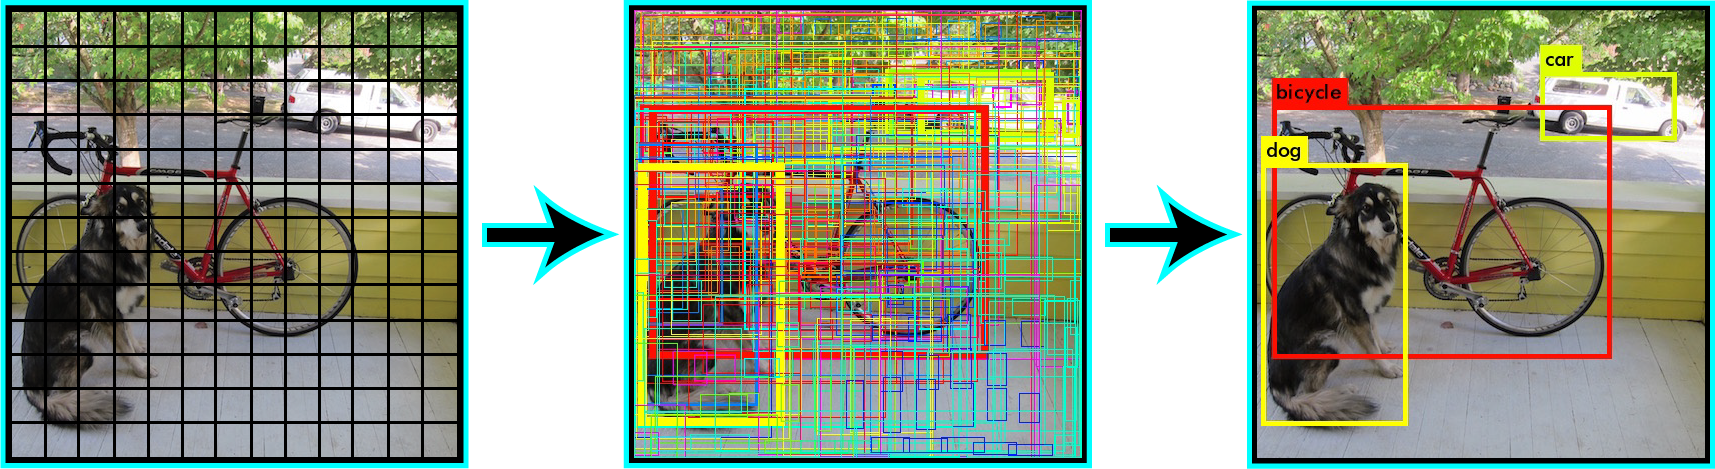
\includegraphics[scale=0.2]{model2.png}
\caption{탐지과정}
\label{fig:detect}
\end{figure}

YOLO 시스템은 분류 기반의 시스템에 비해 몇 가지 장점을 가지고 있다.
그 중 하나는 테스트 시간 동안 전체 이미지를 보고 예측된 정보를 이미지에 텍스트로 알려줍니다. 또한 수천개의 단일 이미지가 필요한 R-CNN 과는 달리 단일 네트워크만으로 평가하고 예측이 가능합니다. 이로 인해 R-CNN보다는 1000배 이상 빠르며 Fast R-CNN보다는 100배 빠릅니다. 전체 시스템에 대한 자세한 내용은 해당 논문\citep{YOLO9000} 을 참고하시기 바랍니다.


\section{탐지기법 실습}

\indent 사전 훈련 된 모델을 사용하여 YOLO 시스템으로 물체를 탐지 하는 방법을 설명합니다. 
Darknet을 아직 설치 하지 않았다면 먼저 설치 해야합니다. \\
이제부터 아래의 명령어를 실행하시기바랍니다.\\
\begin{lstlisting}.
 git clone https://github.com/pjreddie/darknet
 cd darknet 
 make
\end{lstlisting}
실행 후 cfg/ 서브디렉토리에 YOLO에 대한 설정 파일이 존재합니다. 
\\사전 훈련된 가중치를 다운로드한 뒤
\begin{lstlisting}
 wget https://pjreddie.com/media/files/yolo.wegith
\end{lstlisting}
다음을 실행하시기 바랍니다.
\begin{lstlisting}
/darknet detect cfg/yolo.cfg yolo.weights data/dog.jpg 
\end{lstlisting}
여기까지 실행하시면 다음과 같은 출력이 표시됩니다.\\
\begin{lstlisting}
   .layer filters size input output 
   0 conv 32 3 x 3 / 1 416 x 416 x 3 -> 416 x 416 x 32 
   1 max 2 x 2 / 2 416 x 416 x 32 -> 208 x 208 x 32 
   ....... 
   29 conv 425 1 x 1 / 1 13 x 13 x1024 -> 13 x 13 x 425 
   30 detection 
   Loading weights from yolo.weights...Done! 
   data/dog.jpg: Predicted in 0.016287 seconds. 
   car: 54% 
   bicycle: 51% 
   dog: 56% 
\end{lstlisting}

\begin{figure}[h!]
\centering
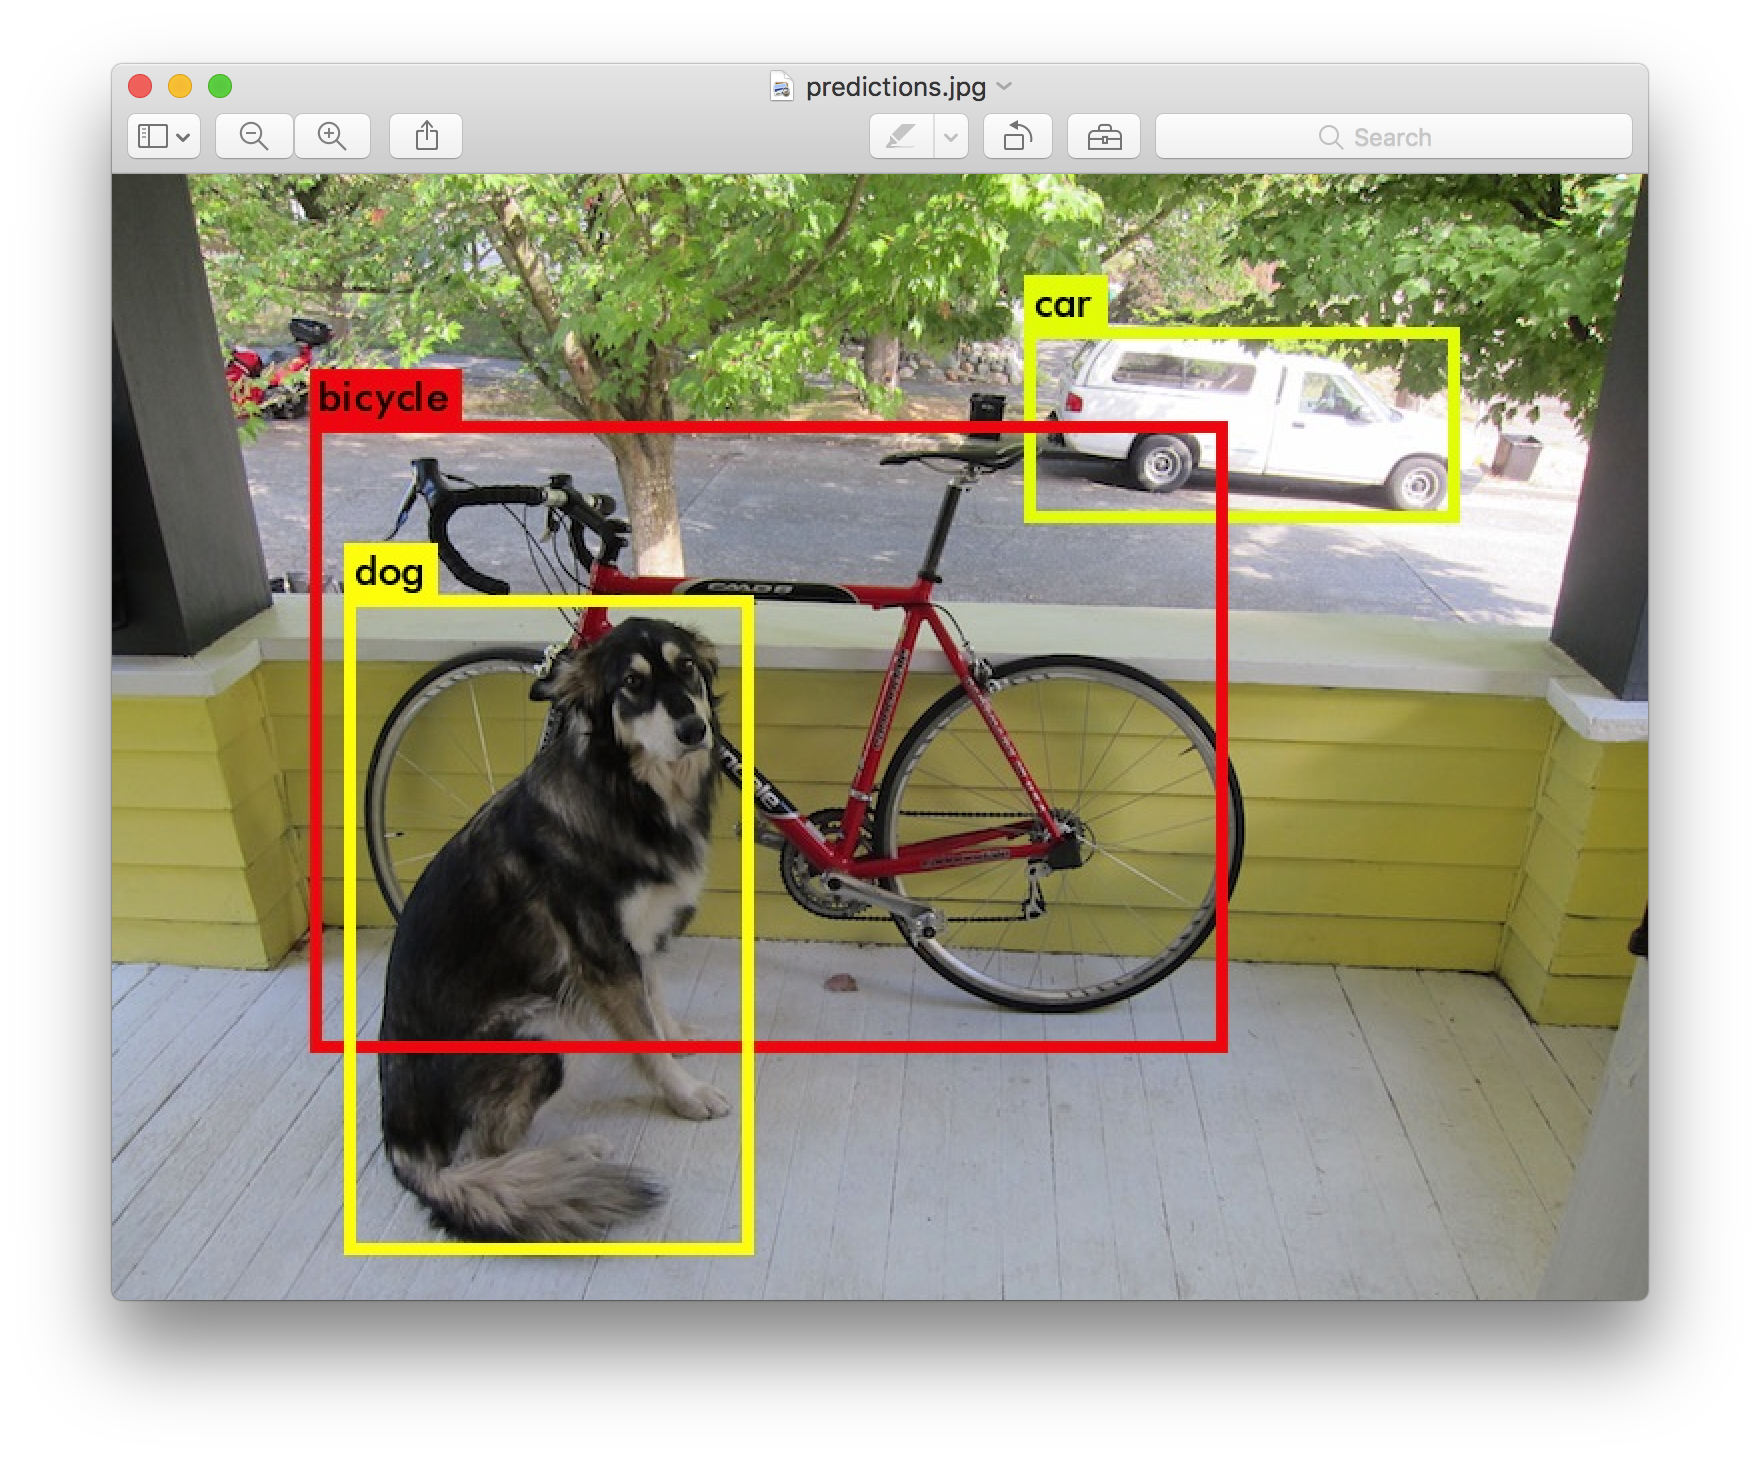
\includegraphics[scale=0.2]{ResultIMAGE.png}
\caption{탐지결과}
\label{fig:result}
\end{figure}

Darknet은 탐지한 객체와 일치도, 발견하는데 소요된 시간을 인쇄합니다.
해당 시스템은 Open CV를 이용해 컴파일하지 않았기 떄문에 탐지를 직접적으로 표시할 수 없습니다. 그렇기에 탐지된 내용을 predictions.png로 저장하고 사용자는 저장된 파일을 열어 탐지된 객체를 확인하는 방식을 사용하고 있습니다. 
해당 시스템은 CPU를 사용하기 때문에 하나의 이미지당 6초에서 12초가 소요됩니다. 
만약 GPU 환경을 사용한다면 더 빨라질 수 있습니다. 이해를 위한 몇 가지 예시 파일들을 포함시켜 놓았습니다. 확인해보시길 바랍니다. \\\\
1. data/eagle.jpg \\
2. data/dog.jpg \\
3. data/person.jpg \\
4. data/horses.jpg\\
\\
detect명령은 보다 일반적인 명령어 버전의 줄임말이며 다음 명령어와 동일합니다.

\begin{lstlisting}
 ./darknet detector test cfg/coco.data cfg/yolo.cfg yolo.weights data/dog.jpg 
\end{lstlisting}

하나의 이미지에서 탐지를 실행하는 시스템이지만 
웹캠에서 실행되는 것과 같은 다른 환경에서의 다른 작업을 수행 할 것인지를 아는 것이 유용하고
앞으로도 배우게 됩니다. 

\section{다중이미지 실습}
명령창에 이미지를 제공하는 대신 하나의 행에 여러 이미지를 시도해 볼 수 있으며 구성과 가중치가 완료되면 프롬포트가 표시됩니다.
\begin{lstlisting}
  ./darknet detect cfg/yolo.cfg yolo.weights 
  layer filters size input output 
  0 conv 32 3 x 3 / 1 416 x 416 x 3 -> 416 x 416 x 32 
  1 max 2 x 2 / 2 416 x 416 x 32 -> 208 x 208 x 32 
  ....... 
  29 conv 425 1 x 1 / 1 13 x 13 x1024 -> 13 x 13 x 425 
  30 detection 
  Loading weights from yolo.weights ...Done! 
  Enter Image Path: 
\end{lstlisting}
data/horses.jpg이미지의 경로를 입력하면 해당 이미지의 경계 영역을 예측하게 됩니다.
\begin{figure}[h!]
\centering
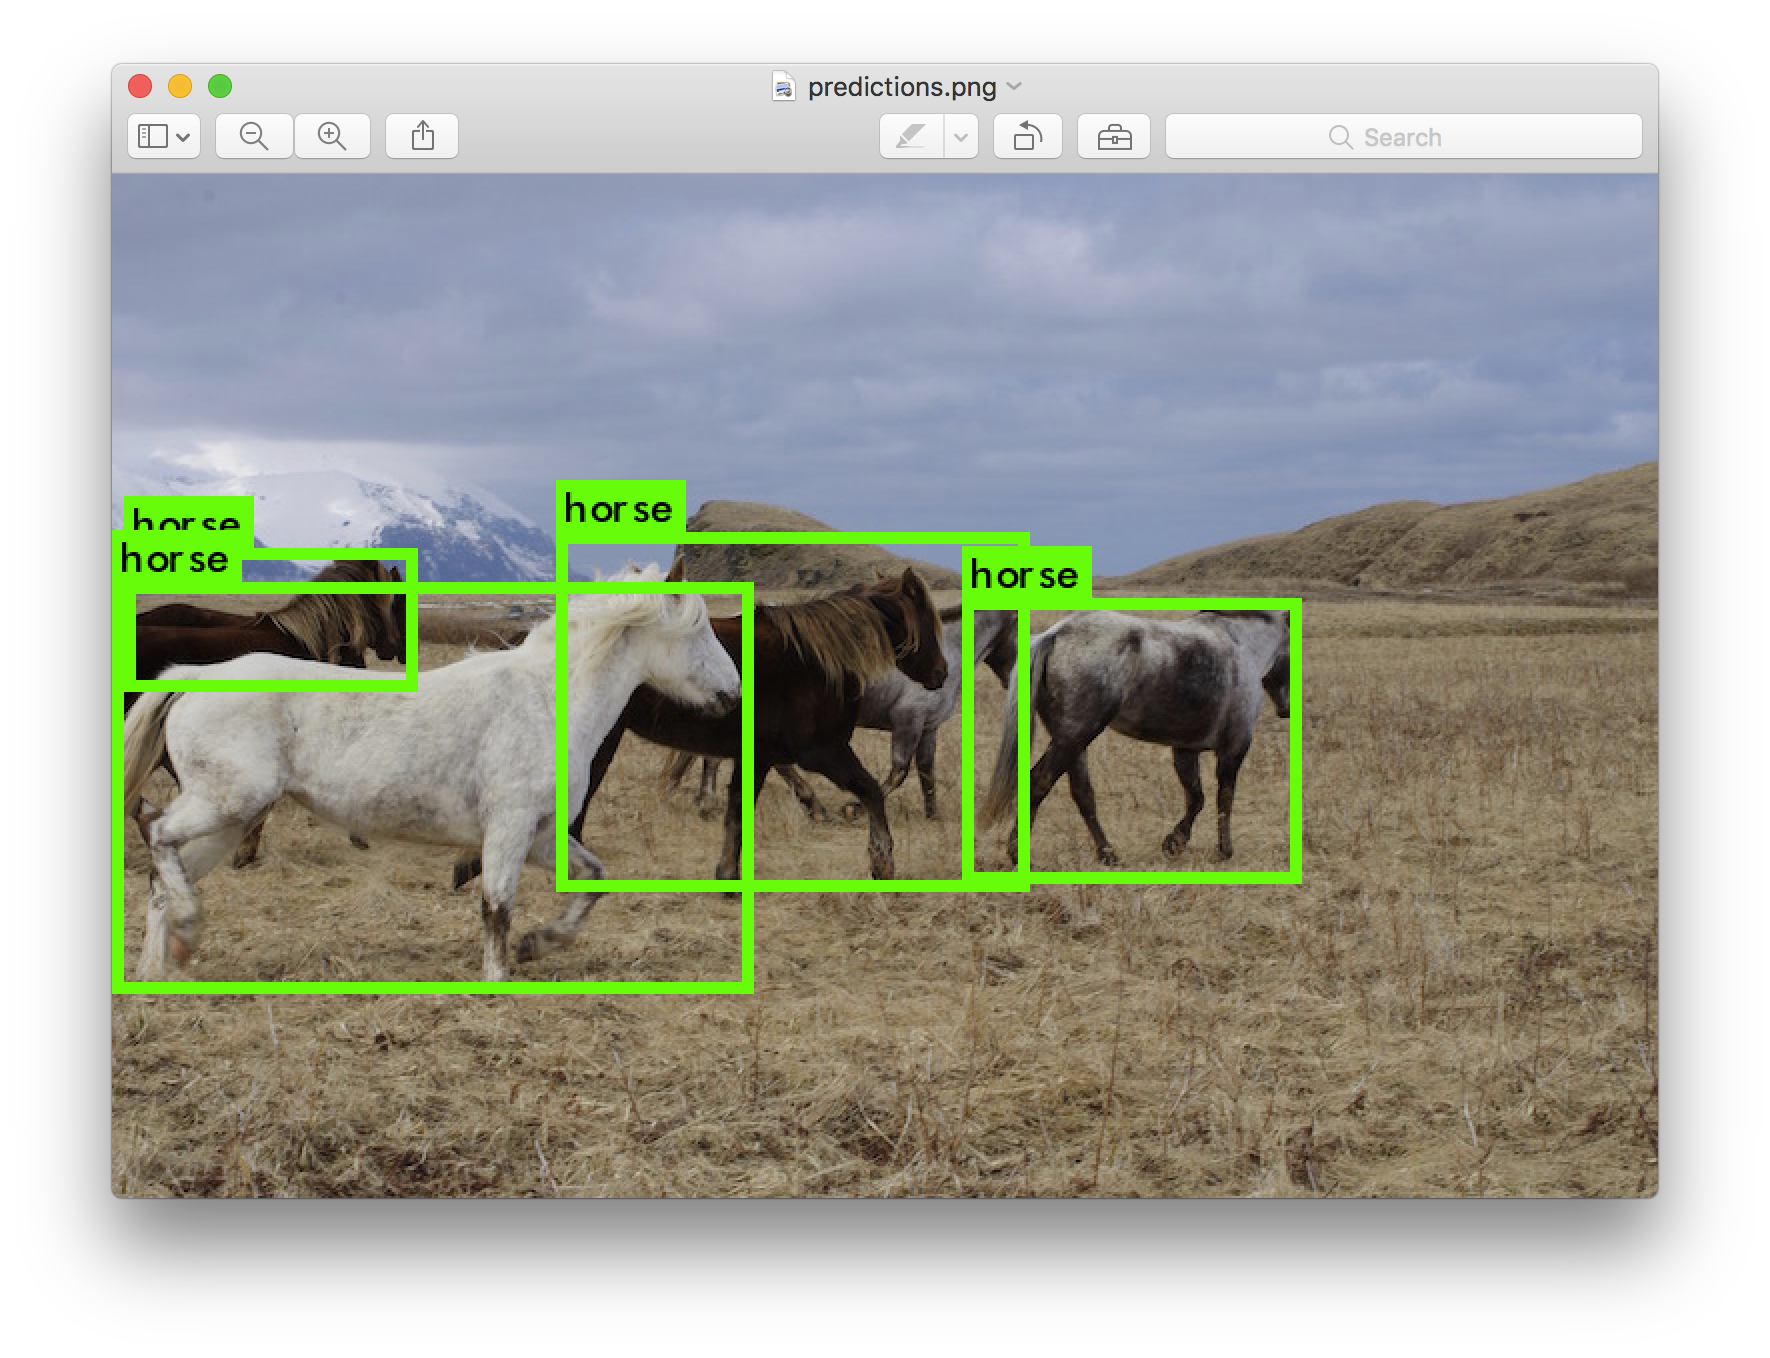
\includegraphics[scale=0.2]{horse.png}
\caption{탐지 결과}
\label{fig:horseresult}
\end{figure}
하나의 이미지가 완료되면 다른 이미지를 시도하귀 위해 더 많은 경로를 물어볼 것입니다.
Ctrl-C를 사용해 프로그램을 종료하시면 됩니다.
\section{탐색의 임계값 변경}
YOLO 시스템의 신뢰도는 기본값이 0.25이며 객체의 탐색 일치도가 0.25 이상인 객체만을 표시하여 사용자에게 보여줍니다.
이러한 임계값은 -thresh <val> 명령어 플래그를 이용하여 임계값을 변경 할 수 있습니다. 
아래의 예시는 탐색된 모든 객체를 표시하기 위하여 임계값을 0으로 설정한 것입니다. 예시 이미지를 참고하시기 바랍니다.
\begin{lstlisting}
 ./darknet detect cfg/yolo.cfg yolo.weights data/dog.jpg -thresh 0 
\end{lstlisting}
\begin{figure}[h!]
\centering
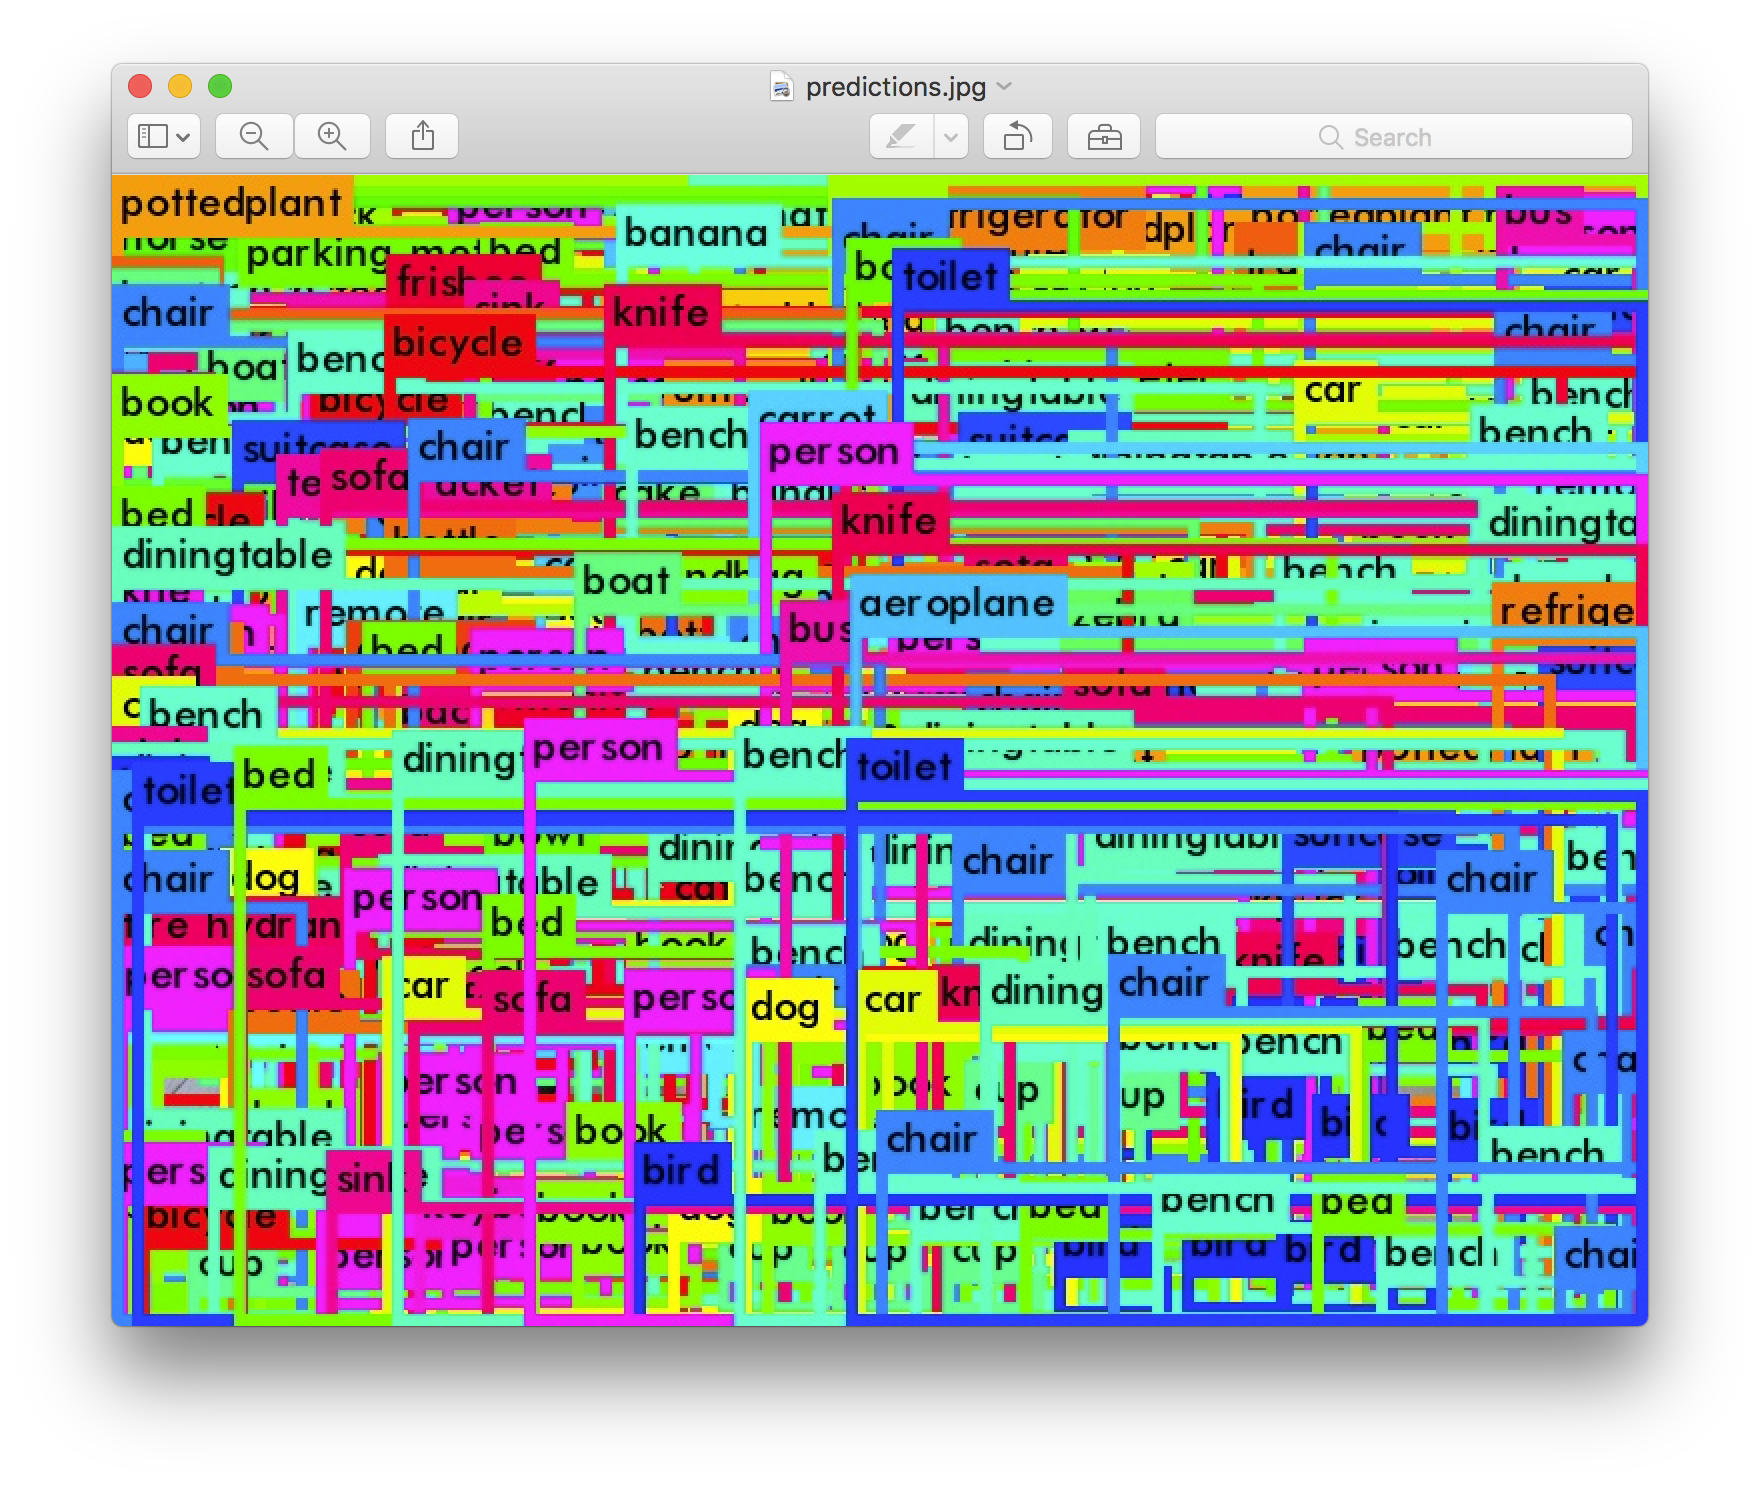
\includegraphics[scale=0.2]{eximage.png}
\caption{임계값 0 탐색결과 }
\label{fig:eximg}
\end{figure}

모델별로 임계값을 제어하는 값을 다른 값으로 설정할 수 있습니다. 
그러나 이것이 유용하다고 명백하게 말하기는 힘듭니다.

\section{TINY YOLO}
Tiny YOLO 시스템은 Darknet reference network를 기반으로 작동하며 일반 YOLO모델보다 훨씬 빠르지만 정확성이 떨어집니다.
VOC에 대한 교육 버전을 사용하려면 다음을 수행하시기 바랍니다.
\begin{lstlisting}
 wget https://pjreddie.com/media/files/tiny-yolo-voc.weights 
 ./darknet detector test cfg/voc.data cfg/tiny-yolo-voc.cfg 
                                             tiny-yolo-voc.weights data/dog.jpg 
\end{lstlisting}

어느 것이 좋고 완벽하다고 자신할 수 없지만 Tiny YOLO 시스템은 확실히 빠릅니다. 
GPU에서는 200 FPS 이상에서 실행이됩니다.
\begin{figure}[h!]
\centering
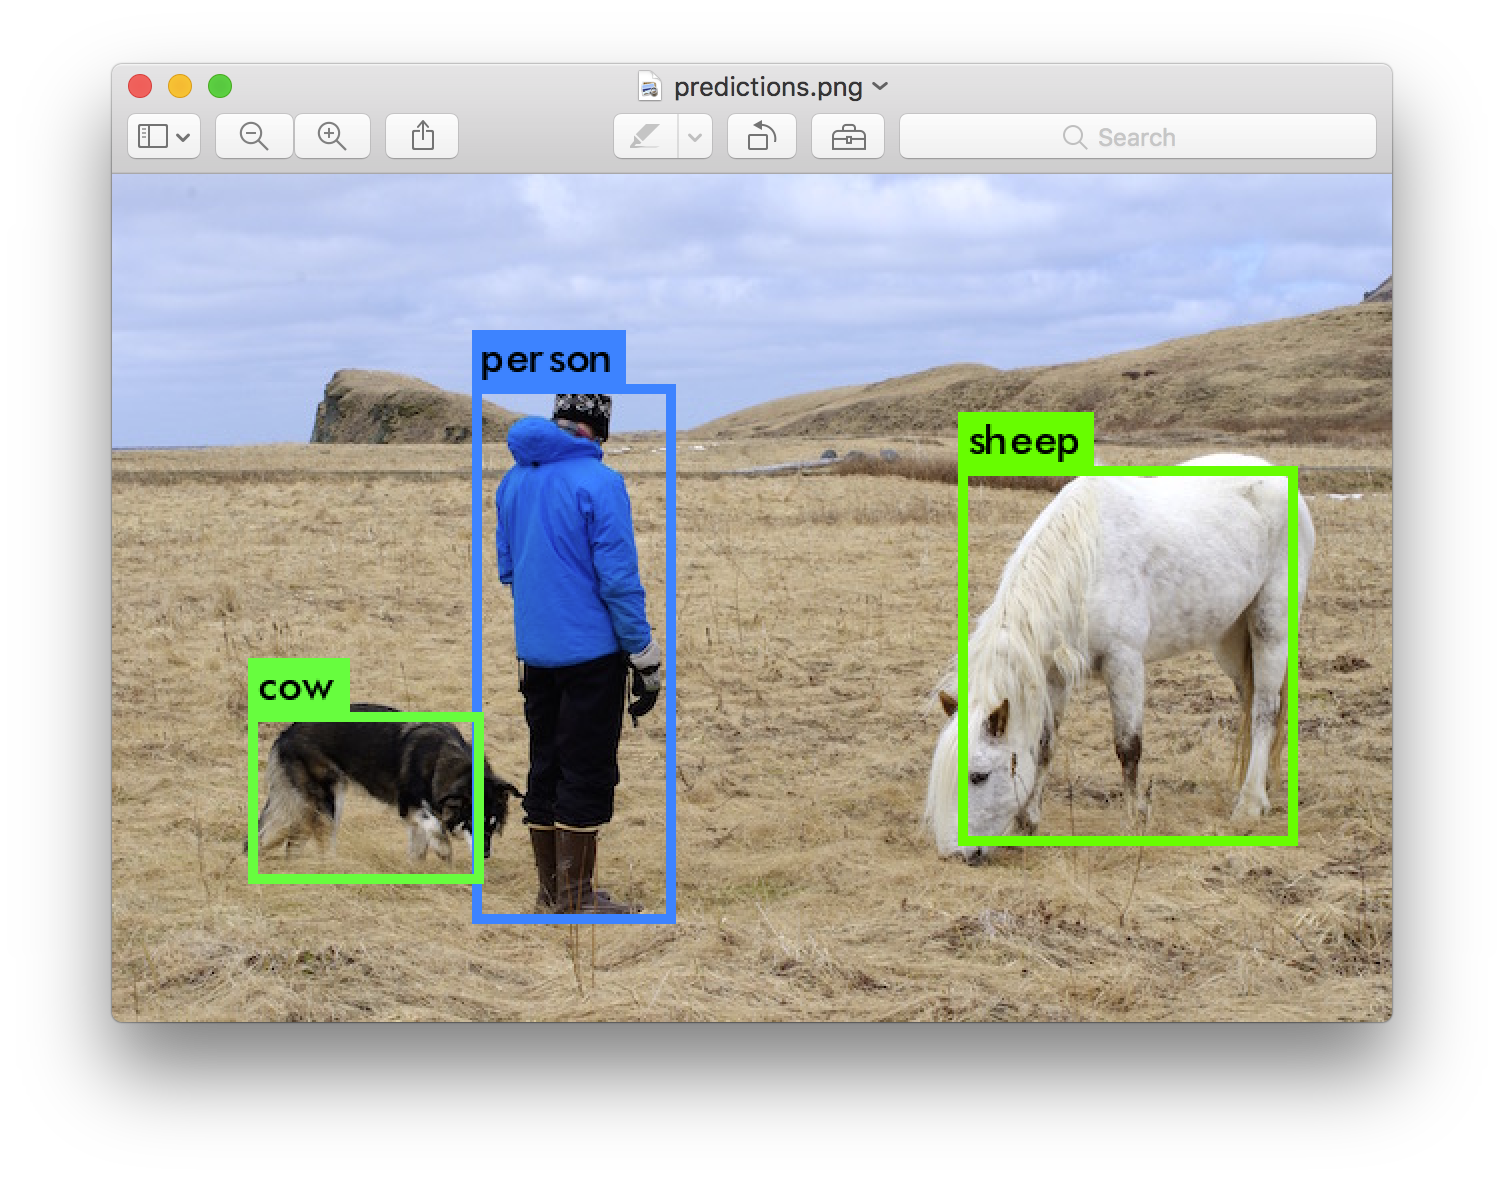
\includegraphics[scale=0.15]{tinyyolo.png}
\caption{임계값 0 탐색결과 }
\label{fig:tinyimg}
\end{figure}

\section{WEBCAM에서의 실시간 탐지}

테스트 데이터에서 YOLO 시스템을 실행하면 결과를 볼 수 없어 흥미롭지 않습니다. 
막대한 이미지 대신 웹캠의 입력으로 실행해 볼 수 있습니다.
Darkent은 CUDA와 OpenCV를 함께 사용하며 이 데모 실행을 위한 컴파일을 해야됩니다. 
다음 명령어를 실행하시기 바랍니다.
\begin{lstlisting}
 ./darknet detector demo cfg/coco.data cfg/yolo.cfg yolo.weights  
\end{lstlisting}
YOLO 시스템은 현재 FPS 및 예상 클래스뿐만 아니라 임계영역이 그려진 이미지를 표시합니다.
OpenCV가 연결할 수있는 컴퓨터에 웹캠이 연결되어 있어야합니다. 그렇지 않으면 작동하지 않습니다. 
여러 웹캠이 연결되어 있고 사용할 웹캠을 선택하려는 경우 -c <num> 입력해 플래그를 전달할 수 있습니다. 
(OpenCV가 사용하는 웹캠의 기본값은 0입니다.) OpenCV가 비디오를 읽을 수 있으면 비디오 파일에서도 실행할 수 있습니다

\begin{lstlisting}
 ./darknet detector demo cfg/coco.data cfg/yolo.cfg yolo.weights <video file> 
\end{lstlisting}
이것이 YOLO 시스템이 위의 YouTube 동영상을 만든 방법입니다

\section{VOC에서의 YOLO 훈련}
다른 훈련체계와 Hyper-Parameters 또는 데이터 셋으로 훈련을 하고 싶다면 YOLO를 처음부터 교육 할 수 있습니다. Pascal VOC 데이터 세트에서 작업하는 방법은 다음과 같습니다.

\section{PASCAL VOC DATA 얻어오기}
YOLO 시스템을 훈련 시키려면 2007 년부터 2012 년까지의 모든 VOC 데이터가 필요합니다. 
여기에서 데이터에 대한 링크(http://khseob0715.dothome.co.kr/YOLO/here.html)를 찾을 수 있습니다. 
모든 데이터를 가져 오려면 모든 디렉토리를 저장하고 해당 디렉토리에서 다음을 실행하시기 바랍니다.
\begin{lstlisting}
  wget https://pjreddie.com/media/files/VOCtrainval_11-May-2012.tar 
  wget https://pjreddie.com/media/files/VOCtrainval_06-Nov-2007.tar 
  wget https://pjreddie.com/media/files/VOCtest_06-Nov-2007.tar 
  tar xf VOCtrainval_11-May-2012.tar 
  tar xf VOCtrainval_06-Nov-2007.tar 
  tar xf VOCtest_06-Nov-2007.tar 
\end{lstlisting}
이제 VOCdevkit/ 하위 디렉토리에 모든 VOC 교육 데이터가 포함되어 있습니다.

\section{VOC에 대한 LABEL 생성}
이제 Darknet이 사용하는 레이블 파일을 생성해야합니다. 
Darknet.txt file with a line for each ground truth object in the image that looks like을 원합니다.
\begin{lstlisting}
  <object-class> <x> <y> <width> <height> 
\end{lstlisting}

여기서 x, y, width, and height 는 이미지의 높이와 너비를 기준으로. 이 파일을 생성하기 위해서
voc label.py Darknet의 스크립트 안에 scripts/ 디렉토리에 있습니다.
그냥 다시 다운로드하는게 안귀찮고 편합니다.
Darknet.txt with a line for each ground truth object in the image that looks like을 원합니다.
\begin{lstlisting}
 wget https://pjreddie.com/media/files/voc_label.py 
 python voc_label.py 
\end{lstlisting}
몇 분 후에이 스크립트는 필요한 모든 파일을 생성합니다. 대부분의 많은 파일 라벨들이 VOCdevkit/VOC2007/labels/ 그리고 VOCdevkit/VOC2012/labels/. 당신의 디렉토리에 가지고 있습니다.
\begin{lstlisting}
 ls 
 2007_test.txt VOCdevkit 
 2007_train.txt voc_label.py 
 2007_val.txt VOCtest_06-Nov-2007.tar 
 2012_train.txt VOCtrainval_06-Nov-2007.tar 
 2012_val.txt VOCtrainval_11-May-2012.tar 
\end{lstlisting}
The text files like 2007 train.txt 와 같은 텍스트 파일은 해당 연도의 이미지 파일과 이미지 세트를 나열합니다. 
DarkNet은 당신이 훈련시키고자 하는 모든 이미지를 가진 하나의 텍스트 파일을 필요로합니다. 이 예제에서
우리 모델을 테스트 할 수 있도록 2007 테스트 세트를 제외한 모든 것을 훈련시켜 봅시다
\begin{lstlisting}
 cat 2007_train.txt 2007_val.txt 2012_*.txt > train.txt 
\end{lstlisting}

이제 우리는 모든 2007 년형 trainval 과 2012 년형 trainval을 하나의 큰 목록에 포함 시켰습니다. 그것이 데이터 설정을 위해해야 할 모든 것입니다!
\section{MODIFY CFG FOR PASCAL DATA}
이제 Darknet 디렉토리로 가십시오. 데이터를 가리 키도록 cfg/voc.data구성 파일을 변경해야합니다.
\begin{lstlisting}
 1 classes= 20 
 2 train = <path-to-voc>/train.txt 
 3 valid = <path-to-voc>2007_test.txt 
 4 names = data/voc.names 
 5 backup = backup 
\end{lstlisting}
<path-to-voc> 을 VOC 데이터를 저장 한 디렉토리로 대체해야합니다.
\section{사전 훈련된 CONVOLUTIONAL 가중치 다운로드}
교육을 위해 우리는 Imagenet에서 사전 훈련 된 Extraction model의 가중치를 사용합니다.
레이어 가중치 다운로드 
\begin{lstlisting}
 wget https://pjreddie.com/media/files/darknet19_448.conv.23 
\end{lstlisting}
사전 훈련 된 가중치를 직접 생성하려면 사전 교육 된 Darknet19 448x448 model 의 다음 명령을 실행하십시오.
\begin{lstlisting}
 ./darknet partial cfg/darknet19_448.cfg darknet19_448.weights 
                                                      darknet19_448.conv.23 23 
\end{lstlisting}
하지만 가중치 파일을 다운로드하면 더 쉽게 사용할 수 있습니다.
\section{모델 훈련}
아래의 명령어를 이용해 훈련을 시킬 수 있습니다.
\begin{lstlisting}
 ./darknet detector train cfg/voc.data cfg/yolo-voc.cfg 
                                                      darknet19_448.conv.23 
\end{lstlisting}

\section{COCO에서의 YOLO 훈련}
만약 다른 훈련체계, Hyper-Parameters 또는 데이터셋을 사용하고 싶다면 YOLO를 처음부터 훈련 시킬 수 있습니다. 
COCO 데이터셋(http://cocodataset.org)에서 작업을 하는 방법은 다음과 같습니다.

\section{COCO DATA 얻어오기}
YOLO 시스템을 훈련시키기 위해서는 모든 COCO의 데이터와 라벨이 필요합니다. 
scripts/get coco dataset.sh 이 스크립트가 해당 작업을 수행합니다. 
COCO 데이터를 넣고 다운로드 하려면 아래를 참고하시면 됩니다.
\begin{lstlisting}
 cp scripts/get_coco_dataset.sh data 
 cd data 
 bash get_coco_dataset.sh 
\end{lstlisting}
이제 Darknet에 모든 데이터와 라벨을 생성해야 합니다.

\section{COCO의 CFG 수정}
이제 Darknet 폴더로 이동합니다. 
cfg/coco.data를 가리키도록 config 파일을 변경해야 합니다.
\begin{lstlisting}
  1 classes= 80 
  2 train = <path-to-coco>/trainvalno5k.txt 
  3 valid = <path-to-coco>/5k.txt 
  4 names = data/coco.names 
  5 backup = backup 
\end{lstlisting}
COCO 데이터를 저장하는 디렉토리로 <path-to-coco>를 대체해야합니다.
또한 cfg를 테스팅 용이 아닌 훈련용으로 수정해야합니다. 
cfg/yolo.cfg가 아래와 같아야 합니다.
\begin{lstlisting}
  [net] 
  # Testing 
  # batch=1 
  # subdivisions=1 
  # Training 
  batch=64 
  subdivisions=8 
  .... 
\end{lstlisting}
\section{모델 훈련}
이제부터 모델 훈련을 위해 아래 명령어를 실행하시기 바랍니다.
\begin{lstlisting}
 ./darknet detector train cfg/coco.data cfg/yolo.cfg 
                                              darknet19_448.conv.23 
\end{lstlisting}
만약 여러개의 GPU를 사용한다면 다음 명령어를 실행하시기 바랍니다.
\begin{lstlisting}
 ./darknet detector train cfg/coco.data cfg/yolo.cfg 
                                              darknet19_448.conv.23 -gpus 0,1,2,3 
\end{lstlisting}
만약 Checkpoint에서 훈련을 중지하고 다시 시작하기 위해서는 다음 명령어를 실행하시기 바랍니다.
\begin{lstlisting}
 ./darknet detector train cfg/coco.data cfg/yolo.cfg 
                                              backup/yolo.backup -gpus 0,1,2,3
\end{lstlisting}
\bibliographystyle{plain}
\bibliography{references}
\end{document}
